%\documentstyle[12pt]{article}
%\documentstyle[psfig,12pt]{article}
%\documentclass[twoside]{article}
%\usepackage{amsmath}
%test compare
\documentclass[11pt]{article}
\usepackage{enumitem}
\setlist{nosep} % or \setlist{noitemsep} to leave space around whole list
\usepackage{bm}
\usepackage{graphicx}
\usepackage{amsmath}
\usepackage{amssymb}
\pagestyle{myheadings} \pagestyle{myheadings}
\renewcommand{\baselinestretch}{1.5}
\setlength{\textheight}{22.5cm}
\setlength{\evensidemargin}{0cm}
\setlength{\oddsidemargin}{0cm}
\setlength{\textwidth}{16.0cm}
\setlength{\headheight}{0cm}
\setlength{\topmargin}{0.5cm}
\newcommand{\be}{\begin{equation}}
\newcommand{\ee}{\end{equation}}
\newcommand{\ba}{\begin{eqnarray}}
\newcommand{\ea}{\end{eqnarray}}
\newcommand{\e}{{\rm e}}
\newcommand{\D}{{\rm d}}

\def\pmb#1{\setbox0=\hbox{#1}%
\kern-.025em\copy0\kern-\wd0
\kern-.05em\copy0\kern-\wd0
\kern-.025em\raise.0433em\box0}

\def \be {\begin{equation}}
\def \ee {\end{equation}}
\def \ba {\begin{array}}
\def \ea {\end{array}}

\def \al {\alpha}

\def \aa {{\bf a}_1}
\def \ab {{\bf a}_2}
\def \bb {{\bf b}_2}

\def \ex {{\bf e}_x}
\def \ey {{\bf e}_y}
\def \ez {{\bf e}_z}

\def \da {\Delta_0}
\def \db {\Delta_1}


\def \kal {k_{\alpha}}
\def \ka {k_a}
\def \kb {k_b}
\def \ko {{\bf k}_0}
\def \kox {k_{0x}}
\def \lam {\lambda}
\def \lap {\bigtriangleup}

\def \vQ {{\bf Q}_p}
\def \vr {{\bf r}}
\def \vR {{\bf R}_p}
\def \u {{\bf u}}
\def \ur {\bf{u}({\bf r})}



\def \x {{\bf x}}


\newcommand{\n}{{\bf n}}
\usepackage[pdftex,unicode,colorlinks, citecolor=blue,%
filecolor=blue, linkcolor=blue, urlcolor=blue]{hyperref}
\usepackage[figure,table]{hypcap} %ссылки на начало рисунка, таблицы...
\begin{document}

%\parskip -20.5pt
\thispagestyle{empty}
\begin{center}
		Assignments for

	\Huge	\textbf{Computations in Physics}
\end{center}
\begin{center}
  by \textit{Victor Zalipaev}, \textit{Aliaksandra Ivinskaya},
  and \textit{Konstantin Ladutenko}\\
  ITMO University
\end{center}
%\parskip 10.5pt

\textbf{Important!} For all problems students have to investigate the result (additionally to `Self Test` subsections), e.g. check the numerical solution against analytic one, check the dependence of the resulting error against mesh, domain size, source and monitor points positions (if any), etc. `Self Test` subsections are just hints for possible directions of research.

There are four modules (PDE with FD, FDTD, FDFD, and FEM), problems in each module should be solved in sequence.

\section{Solving PDE with finite differences}

Solve 2D Dirichlet boundary value problem

 \be
\left \{\begin{array}{ll}\frac{\partial^2u}{\partial
x^2}+\frac{\partial^2u}{\partial
y^2}=0,~~~~~{\rm in}~~~ \Omega,\\
u|_{\partial\Omega}=\phi,~~~~~{\rm on}~~~\partial\Omega.
\end{array} \right. \label{dp}
 \ee
using finite difference method, where $\Omega$ is a rectangle with
$x\in[0,a]$ and $y\in[0,b]$.

\subsection{Iterative solver}
\label{sec:iterative-solver}

Use iterative method (explicit scheme with finite differences) to solve 2D
Dirichlet boundary value problem (1) with the following boundary
conditions
 \be
 \left \{\begin{array}{ll}
\phi(x,0)=0,~~~\phi(x,b)=\sin(x)/\sin(a),~~~x\in[0,a] \\

\phi(0,y)=0,~~~\phi(a,y)=\sinh(y)/\sinh(b),~~~y\in[0,b].
 \end{array} \right. \label{bc}
 \ee

\textbf{Self Test:}
\begin{enumerate}
\item Compare against an analytic solution.
\begin{enumerate}
\item Check the convergence depending on the mesh size and the number of Jacobi iterations.
\item Plot a color map with numerical and analytic solutions, and the difference (error).
\item Plot a root-mean-square of the error vs mesh step. Check it for several domain sizes.
\end{enumerate}
\item Increase $a$ twice, keep $b$ the same. Run simulation, explain the result.
\item Change the boundary condition to become discontinuous.  Run simulation, explain the result.
\item Check the evaluation time dependence on mesh size and number of iterations.
\item (Optional) Check the evaluation speed difference when using nested cycles, sections of NumPy arrays, and Numba JIT compilation in your Python implementation.
\end{enumerate}



\subsection{Inverse matrix method}
\label{sec:inverse-matr-meth}

Use the inverse matrix method to solve the corresponding linear system
of algebraic equations in order to find finite difference solution
to the Dirichlet boundary value problem (1) with the following
boundary conditions (\ref{bc}).

\textbf{Self Test:}
\begin{enumerate}
\item Compare the results with ones obtained from Jacobi iterative solver.
\item (Optional) Compare the evaluation time and memory consumption with an iterative solver depending on mesh size. Try several matrix solvers (e.g. inverting the full matrix, using sparse matrix generalized minimal residual iteration solver, etc.).
\end{enumerate}

\subsection{Heat transfer equation}


Solve the initial-boundary problem for the heat transfer equation
 $$ \frac{\partial u}{\partial t}=\frac{\partial^2u}{\partial
x^2},~~~~~ u(x,0)=\sin(\pi x),~~~~~0\le x\le 1,~~~~~
u(0,t)=u(1,t)=0,~~~~~t\ge 0.
 $$
 Use the generalized Crank-Nicolson finite-difference method with
 $\theta=0$ (explicit scheme), $\theta=1$ (implicit scheme), and
 $\theta=1/2$ (Crank-Nicolson scheme) for a different ratio between
 steps in $x$ and $t$.

 \textbf{Self Test:}
\begin{enumerate}
\item Compare against the exact solution for all schemes. Check the stability and accuracy depending on Courant number.
\item Check the solution accuracy behavior depending on $t_{max}$ for all schemes.
 \end{enumerate}


\subsection{Wave equation}
\label{sec:wave-equation}


Solve the initial-boundary problem for the wave  equation
 $$ \frac{\partial^2 u}{\partial t^2}=\frac{\partial^2u}{\partial
x^2},~~~~~ u(x,0)=\sin(\pi x),~~~~~u_t(x,0)=\sin(\pi x),
 $$
 $$
0\le
x\le 1,~~~~~ u(0,t)=u(1,t)=0,~~~~~t\ge 0.
 $$
 Use the finite-difference method with explicit
 scheme for a different ratio between steps in $x$ and $t$.

 \textbf{Self Test:}
\begin{enumerate}
\item Compare against the exact solution. Check the stability and accuracy depending on Courant number. What is the optimal value of Courant number?
 \end{enumerate}


\section{FDTD}

All FDTD simulations are expected to be one-dimensional. For plotting multiply the magnetic field to the impedance of free space.

Recommended books:
\begin{itemize}
  \item (easy) Understanding the Finite-Difference Time-Domain Method,
	   John B. Schneider, \url{www.eecs.wsu.edu/~schneidj/ufdtd}, 2010. (it is
    also available at GitHub \url{https://github.com/john-b-schneider/uFDTD} )
  \item (medium) Numerical electromagnetics : the FDTD method / Umran
    S. Inan, Robert A. Marshall. 2011
  \item (full) A. Taflove and S. C. Hagness, Computational
    Electrodynamics: The Finite-Difference Time-Domain Method, 3rd
    ed. Norwood, MA: Artech House, 2005.
  \end{itemize}

  Implementation examples: \url{https://github.com/kostyfisik/fdtd-1d}


\subsection{Vanish electric field in vacuum\label{sec:vanish-e-field}}
Simulate a system with magnetic mirror boundary condition ($H=0$) on
one side and electric mirror ($E= 0$) on the other side. The source of
the electric field has a Gaussian profile in time, it is located exactly
in the center of the simulated domain. Wave is propagating from the
source to the boundaries and back. The successful presentation should
provide a sequence of images as a time evolution (or animation) for
electric and magnetic fields. The simulation should finish at the
moment where the electric field vanishes (all energy is in the
magnetic field).

\textbf{Self Test:}
\begin{enumerate}
\item  Which boundary of the domain is an electric mirror and why?
\item What is the Yee cell and Yee algorithm? What is the reason to use it in space and time?
\item What is the reason for the wave to travel away from the source
  (from a physical and numerical point of view)? In a 1D simulation, this
  means that just after the excitation wave located left to the source goes to
  the left and wave located right to the source goes to the
  right.
\item What is the number of field components being updated every time step?
\item Why magnitude of electric field at the end of
  the simulation is not an exact zero? How the reminding ``noise''
  can be increased? How it can be decreased?
\item Run a simulation using the source time-profile to be one half of
  the Gaussian curve (with an abrupt change of the amplitude). What is the reason for the flutter? How it can
  be fixed? Why? What will happen if we increase the mesh density? \underline{Hint:} To provide a correct answer you should
  understand the origin of Courant condition, provide a Fourier image
  of a Gaussian profile, qualitatively explain how it will change the
  Fourier image when the half of Gaussian profile is cropped out.
\item  What will happen if you use a Heaviside step function as a source? Why?
\item  What you should put into your code to introduce a
  magnetic dipole source? How can you prove that it is really a
  magnetic dipole?
\end{enumerate}

\subsection{Simple ABC\label{sec:simple-abc}}

Simulate a system with a simple absorbing boundary condition (ABC) as it
is defined in \href{http://www.eecs.wsu.edu/~schneidj/ufdtd/}{J.B.~Schneider book}, section \href{https://github.com/john-b-schneider/uFDTD/blob/b17f574631d5ffdf1167f23aa7bc74a6819fd171/fdtd-intro.tex#L1039}{ ``Terminating the
  Grid''}.
The source of the electric field has a Gaussian profile in time; it is
located exactly in the center of the simulated domain (same as in~\ref{sec:vanish-e-field}). The successful
presentation should provide a sequence of images as a time evolution (preferred) or animation (with an ability to skip initial part of the simulation and to pause at any given moment for visual investigation of result) for electric and magnetic fields before and after the
wave hits the boundary.

\textbf{Self Test:}
\begin{enumerate}
\item Explain, why does simple ABC works as expected? Which lines in
  the code represent simple ABC?
\item Use the host media with the refractive index $n=2$ for the same
  simulation. You should observe the increase of reflection from the
  boundary. Why does it happen? How it can be fixed? (provide at least two code samples using different approaches)
\end{enumerate}

\subsection{Mur ABC}
\label{sec:mur-abc}
Same as~\ref{sec:simple-abc} using Mur ABC.

\textbf{Self Test:}
\begin{enumerate}
\item Explore Mur ABC performance (amplitude ratio of the incident and
  the reflected wave from the boundary) in a wide range of refractive
  index values and the source parameters. Why does Mur ABC perform
  better compared to simple ABC?
\item Sometimes you can observe the distortion of the Gaussian field
  profile propagating in the media (short pulses on coarse mesh). What this simulation conditions lead to distortion?
\item Name few other types of ABC.
\end{enumerate}

\subsection{CPML}
\label{sec:cpml}

Same as~\ref{sec:simple-abc} using convolution perfectly matched layer (CPML) as a boundary condition.

\textbf{Self Test:}
\begin{enumerate}
\item Compare Mur ABC with 5, 10, and 20 cells of PML for few values of host media index.
\item What is the difference of CPML compared to Berenger PML, UPML, CFS-PML, etc? Which one you should select depending on the model under consideration?
\item Find out in the literature the benefits of PML over ABC (including 2D and 3D cases). \underline{Hint:} Consider evanescent waves, discursive and non-linear media, etc.
\item Why PML performance is low for 5 cell? How does it depend on
  total PML width and why?  What it the principal difference for usage of the polynomial or geometric grading for conductivity in the PML?
\item PML is perfectly matched by impedance with free space. Why we
  need to use grading of conductivity in the PML to make it work?
  \underline{Hint:} The answer is related to Yee grid.
\end{enumerate}

\subsection{Fresnel equation}
\label{sec:fresnel-equation}
Compare against Fresnel equations
\verb+http://en.wikipedia.org/wiki/Fresnel_equations+ , find the limits of
FDTD applicability.

\textbf{Self Test:}
\begin{enumerate}
\item What is the origin of the difference between numerical (from
  FDTD) and analytic solution?
\item How does numerical error depend on boundary conditions? Is it
  possible to remove this dependence?
\item Check the dependence of error on the position of monitor point (including points near the boundary and the interface).
\item How does the numerical error depend on the refractive index of  each of two materials? How the numerical error can be reduced? \underline{Hint:} consider the influence of Courant number.
\end{enumerate}


\subsection{Dielectric slab}

Compare FDTD results against a single dielectric slab (e.g
http://www.ece.rutgers.edu/~orfanidi/ewa/ch05.pdf), you should provide
simulation of reflection-less cases of a quarter-wavelength and
half-wavelength width  slab.

\textbf{Self Test:}
\begin{enumerate}
\item In the provided task examples we use \verb+int()+ function to set the
  refractive index of the slab. Why do we need it? How we can avoid
  using \verb+int()+ function?
\item Why does the reflection from the non-reflecting slab depends on
  boundary conditions?
\item What is the difference between quater-wavelength and
  half-wavelength slab from the numerical error point of view?
\item (optional) Plot a transmission spectra from a single simulation run. \underline{Hint:} Use a short pulse to cover the spectral range of interest and discrete Fourie transform $$F(f) = \Delta t \sum_{m=1}^M \left(e^{-j 2 \pi f \Delta t}\right)^m f(m),$$ where $f(m)$ field values at given time-step. Perform the summation via the main loop (so, no need to store field time-profile). Compare the performance, when expression in round brackets is evaluated inside of loop or computed in advance.
\end{enumerate}

\section{FDFD}

To read: presentation Course\_FDFD.pdf at \url{https://github.com/kostyfisik/fdfd-1d}

\subsection{PEC-PMC cavity}
\label{sec:pec-pmc-cavity}
\begin{itemize}
\item Find the modes of the PMC-PEC cavity.
\item Check how solution improves as discretization becomes finer.
\item Visualize the field inside the cavity.
\end{itemize}

\underline{Hint:} A good example is available from 2016 year student
Pavel Dmitriev \url{https://github.com/kostyfisik/students-2018/blob/p.dmitriev/2_fdfd/Task1_PEC-PMC_Eigenmodes.ipynb}

\textbf{Self Test:}
\begin{enumerate}
\item Check field dependence on discretization (phase
  and amplitude), explain the result.
\item How the boundary condition is applied?
\item (Optional) Check memory consumption and performance when using sparse and full matrix representation of the problem depending on the mesh size.
\end{enumerate}

\subsection{Multilayer band gap (BG) diagram}
\label{sec:multilayer-band-gap}

Build 1D BG diagram for a multilayer consisting of two dielectrics of
$\varepsilon_1$ and $\varepsilon_2$. Assume the layers have equal
thickness. See how BG opens as the contrast between $\varepsilon_1$ and
$\varepsilon_2$ increases.

\section{FEM}

To read: \url{https://github.com/kostyfisik/fem-intro}

\subsection{Quadratic elements}
\label{sec:quadratic-elements}

Solve 1D Poisson's equation using FEM with quadratic elements.

\textbf{Self Test:}
\begin{enumerate}
\item Compare against the analytic solution, change the number of elements.
\item Plot on the same figure the solution and shape functions multiplied by wight for each element.
\item What is the main idea of the Galerkin method?
\end{enumerate}

\subsection{(optional) Scattering on infinite cylinder}
Evaluate electric field for the scattering on $TM^z$ plane wave on PEC infinite cylinder using Fenics Project FEM library \url{https://fenicsproject.org/}. \underline{Hint:} After getting acquainted with Fenics tutorial \url{https://fenicsproject.org/tutorial/} use the mathematical statement of the problem from  Anastasis C. Polycarpou book ``Introduction to the Finite Element Method in Electromagnetics'' sec. 2.10.2 to solve the problem in Python.

\textbf{Self Test:}
\begin{enumerate}
\item Compare against the analytic solution, change the number of elements and the order of approximation.
\end{enumerate}

\newpage
\section*{Solving}

 

\section*{Solving}

We have system of PDE.

And If used explicit method we obtain 

\begin{equation}
    u_{i, j} = \frac{1}{4} (u_{i+1,j} + u_{i-1,j} + u_{i,j+1} + u_{i,j-1}) 
\end{equation}

\begin{figure}[h!]
\centering{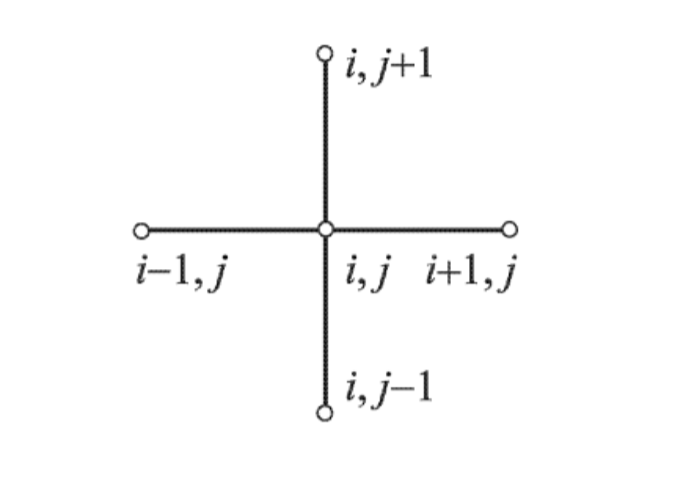
\includegraphics[scale=0.4]{1_1_numerical.png}}
\caption{explicit method}
\end{figure}




\end{document}
